\section{Početni zaslon i glavna navigacija}

Nakon uspješne prijave na mobilnoj aplikaciji, korisnik pristupa početnom zaslonu koji je dizajniran kao personalizirana kontrolna ploča. (slika~\ref{fig:početni_zaslon})

\begin{figure}[H]
    \centering
    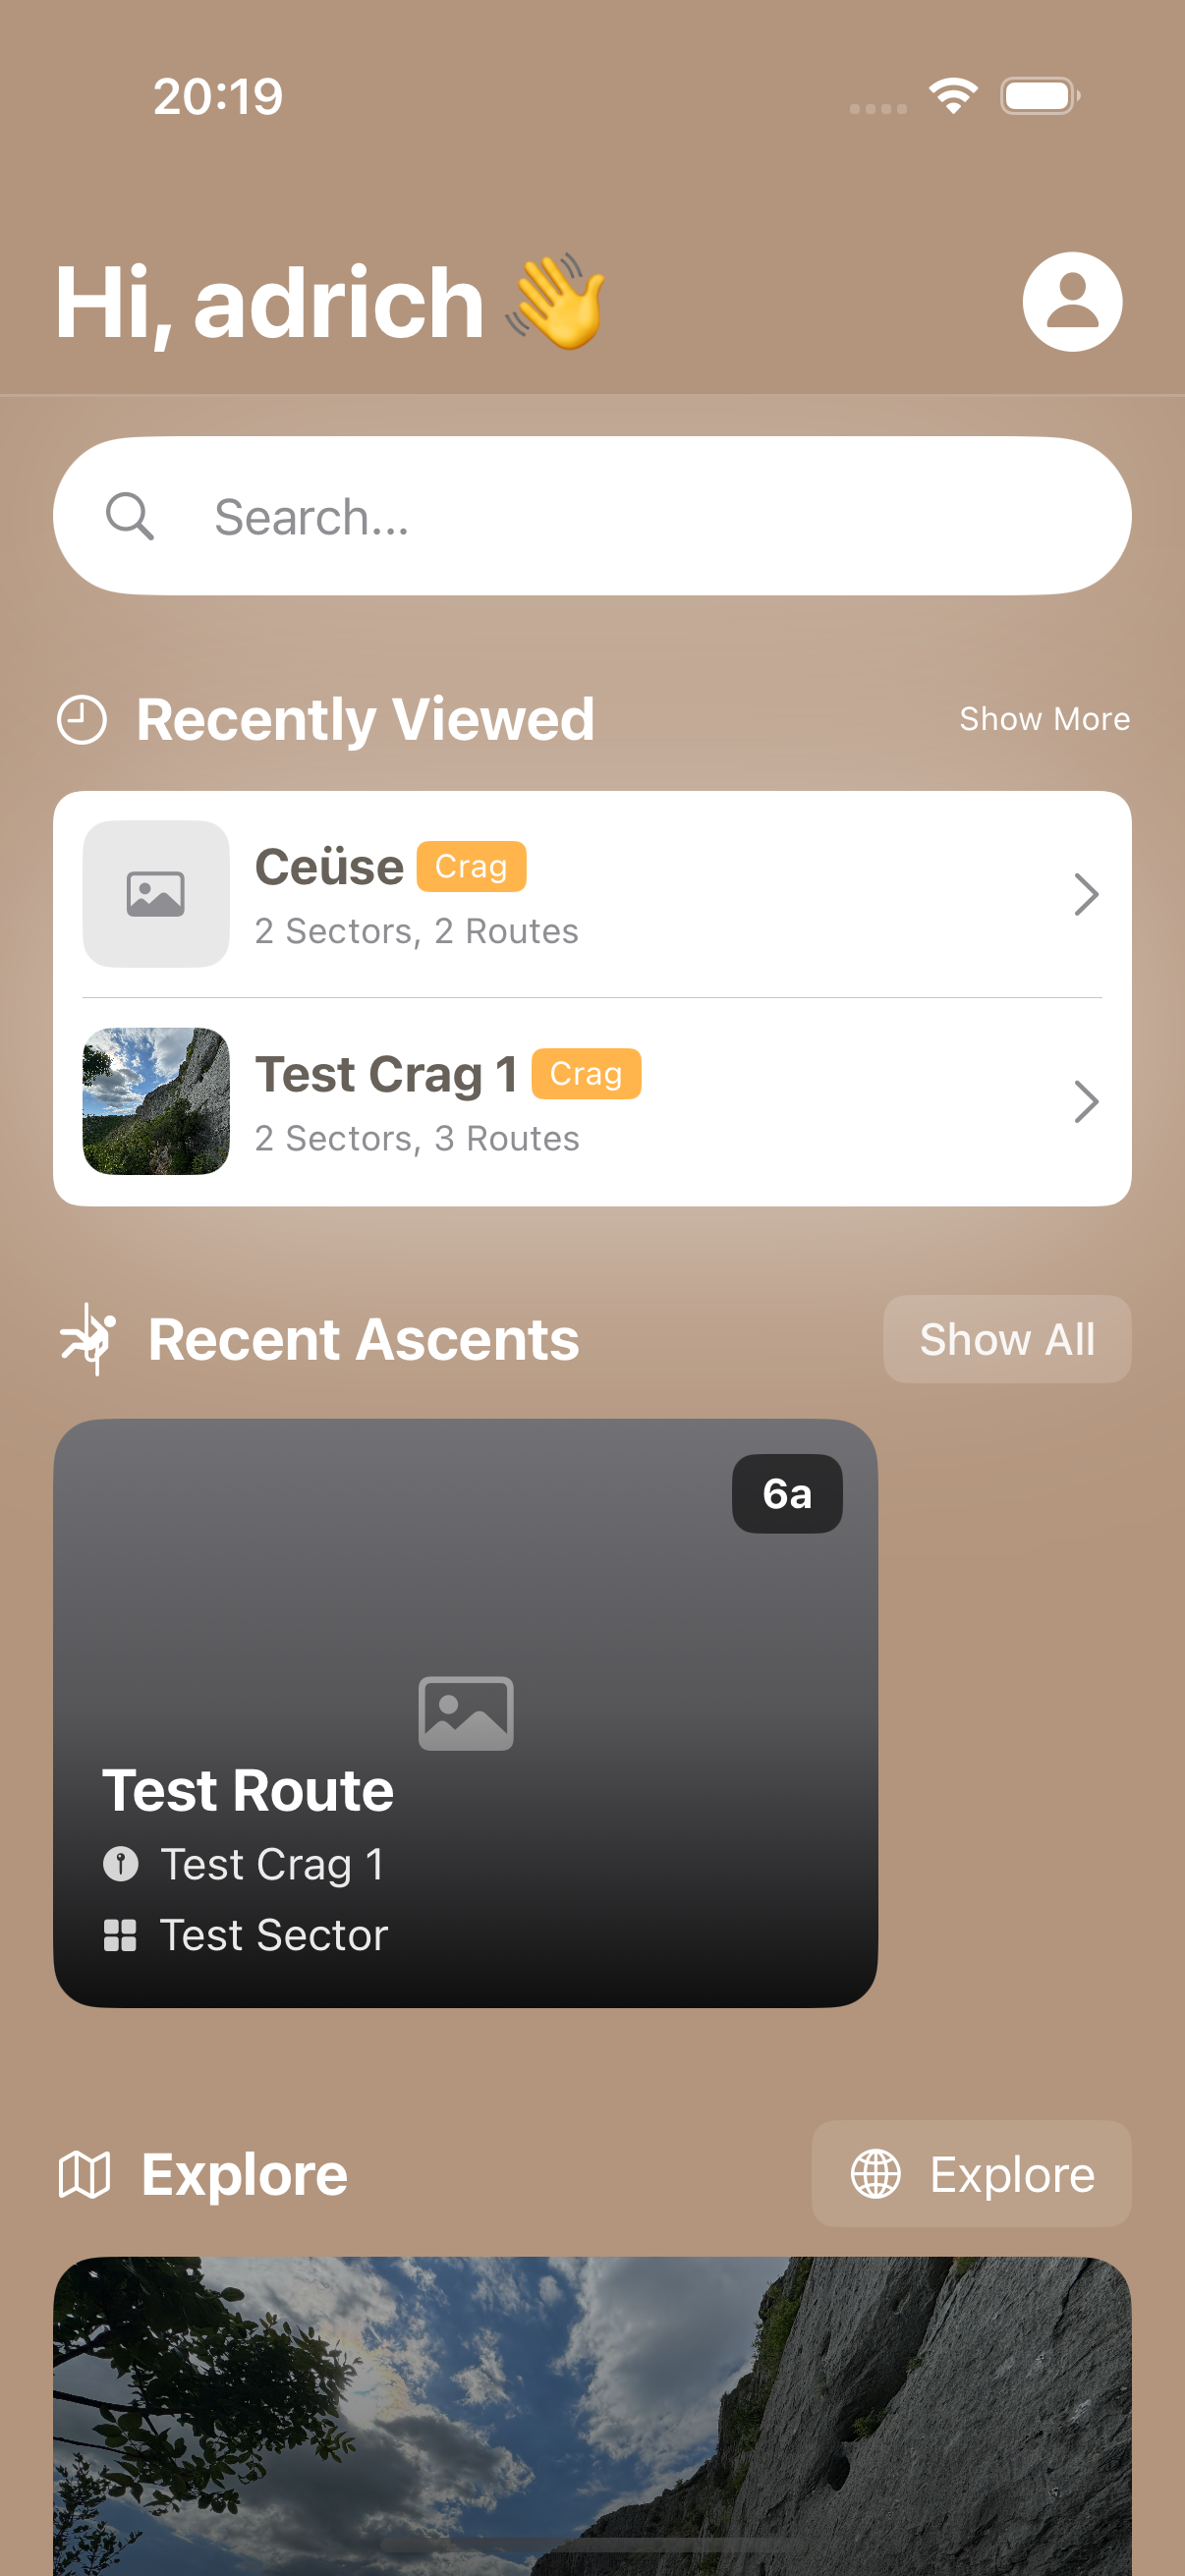
\includegraphics[width=0.35\textwidth]{images/implementacija/main_nav_1.png}
    \caption{Navigacijski zaslon aplikacije "Alpinity"}
    \label{fig:početni_zaslon}
\end{figure}

Ovaj zaslon omogućuje brzi pristup najvažnijim informacijama i funkcionalnostima. Zaslon je organiziran u nekoliko cjelina. Na vrhu zaslona nalazi se personalizirana dobrodošlica, gumb koji vodi korisnika na detalje korisničkog profila te istaknuto polje za pretraživanje koje omogućuje brzu i direktnu pretragu svih penjališta, sektora, penjačkih smjerova i korisnika.

Sekcija "Nedavno pregledano" (eng. \textit{Recently viewed}) nudi brze poveznice na detalje penjališta, sektore, penjačke smjerove i drugih korisnika koje je korisnik nedavno pregledavao. Korisnik ima opciju "Vidi više" (eng. \textit{View more}) koja nudi korisniku prikaz više poveznica koje je posjetio.

Odmah ispod, u sekciji "Nedavni usponi" (eng. \textit{Recent ascents}) nalazi se lista najnovijih uspona korisnika zabilježenih u dnevniku uspona. Pritiskom na određeni element liste otvara se pregled detalja tog penjačkog smjera. Klikom na "Pokaži sve" (eng. \textit{Show all}) otvara se pregled vlastitog profila gdje su zapisani svi korisnikovi usponi. 

Na dnu zaslona nalazi se sekcija "Istraži" (eng. \textit{Explore}) namijenjena otkrivanju novih penjališta pomoću prijedloga popularnih penjališta. Preporuke su određene u odnosu na prijašnje korisnikove uspone, specifično preporuke su penjališta koje se nalaze u blizini penjališta koje je korisnik nedavno posjetio. Klikom na određeno penjalište u listi odlazi se na pregled detalja tog penjališta. Pritiskom na gumb "Istraži" (eng. \textit{Explore}) otvara se pregled sa geografskom kartom sa svim penjališta.

Na web aplikaciji ne postoji ekvivalent za početni zaslon mobilne aplikacije, već poveznice na nedavno pregledane entitete nalaze se u sklopu pretraživanja. Nedavni usponi su dostupni u sklopu stranice korisničkog profila, a "Istraži" sekcija je pretvorena u zasebnu stranicu koja sadrži geografsku kartu sa penjalištima i prijedlozima popularnih penjališta (slika~\ref{fig:istrazivanje_web}).

\begin{figure}[H]
    \centering
    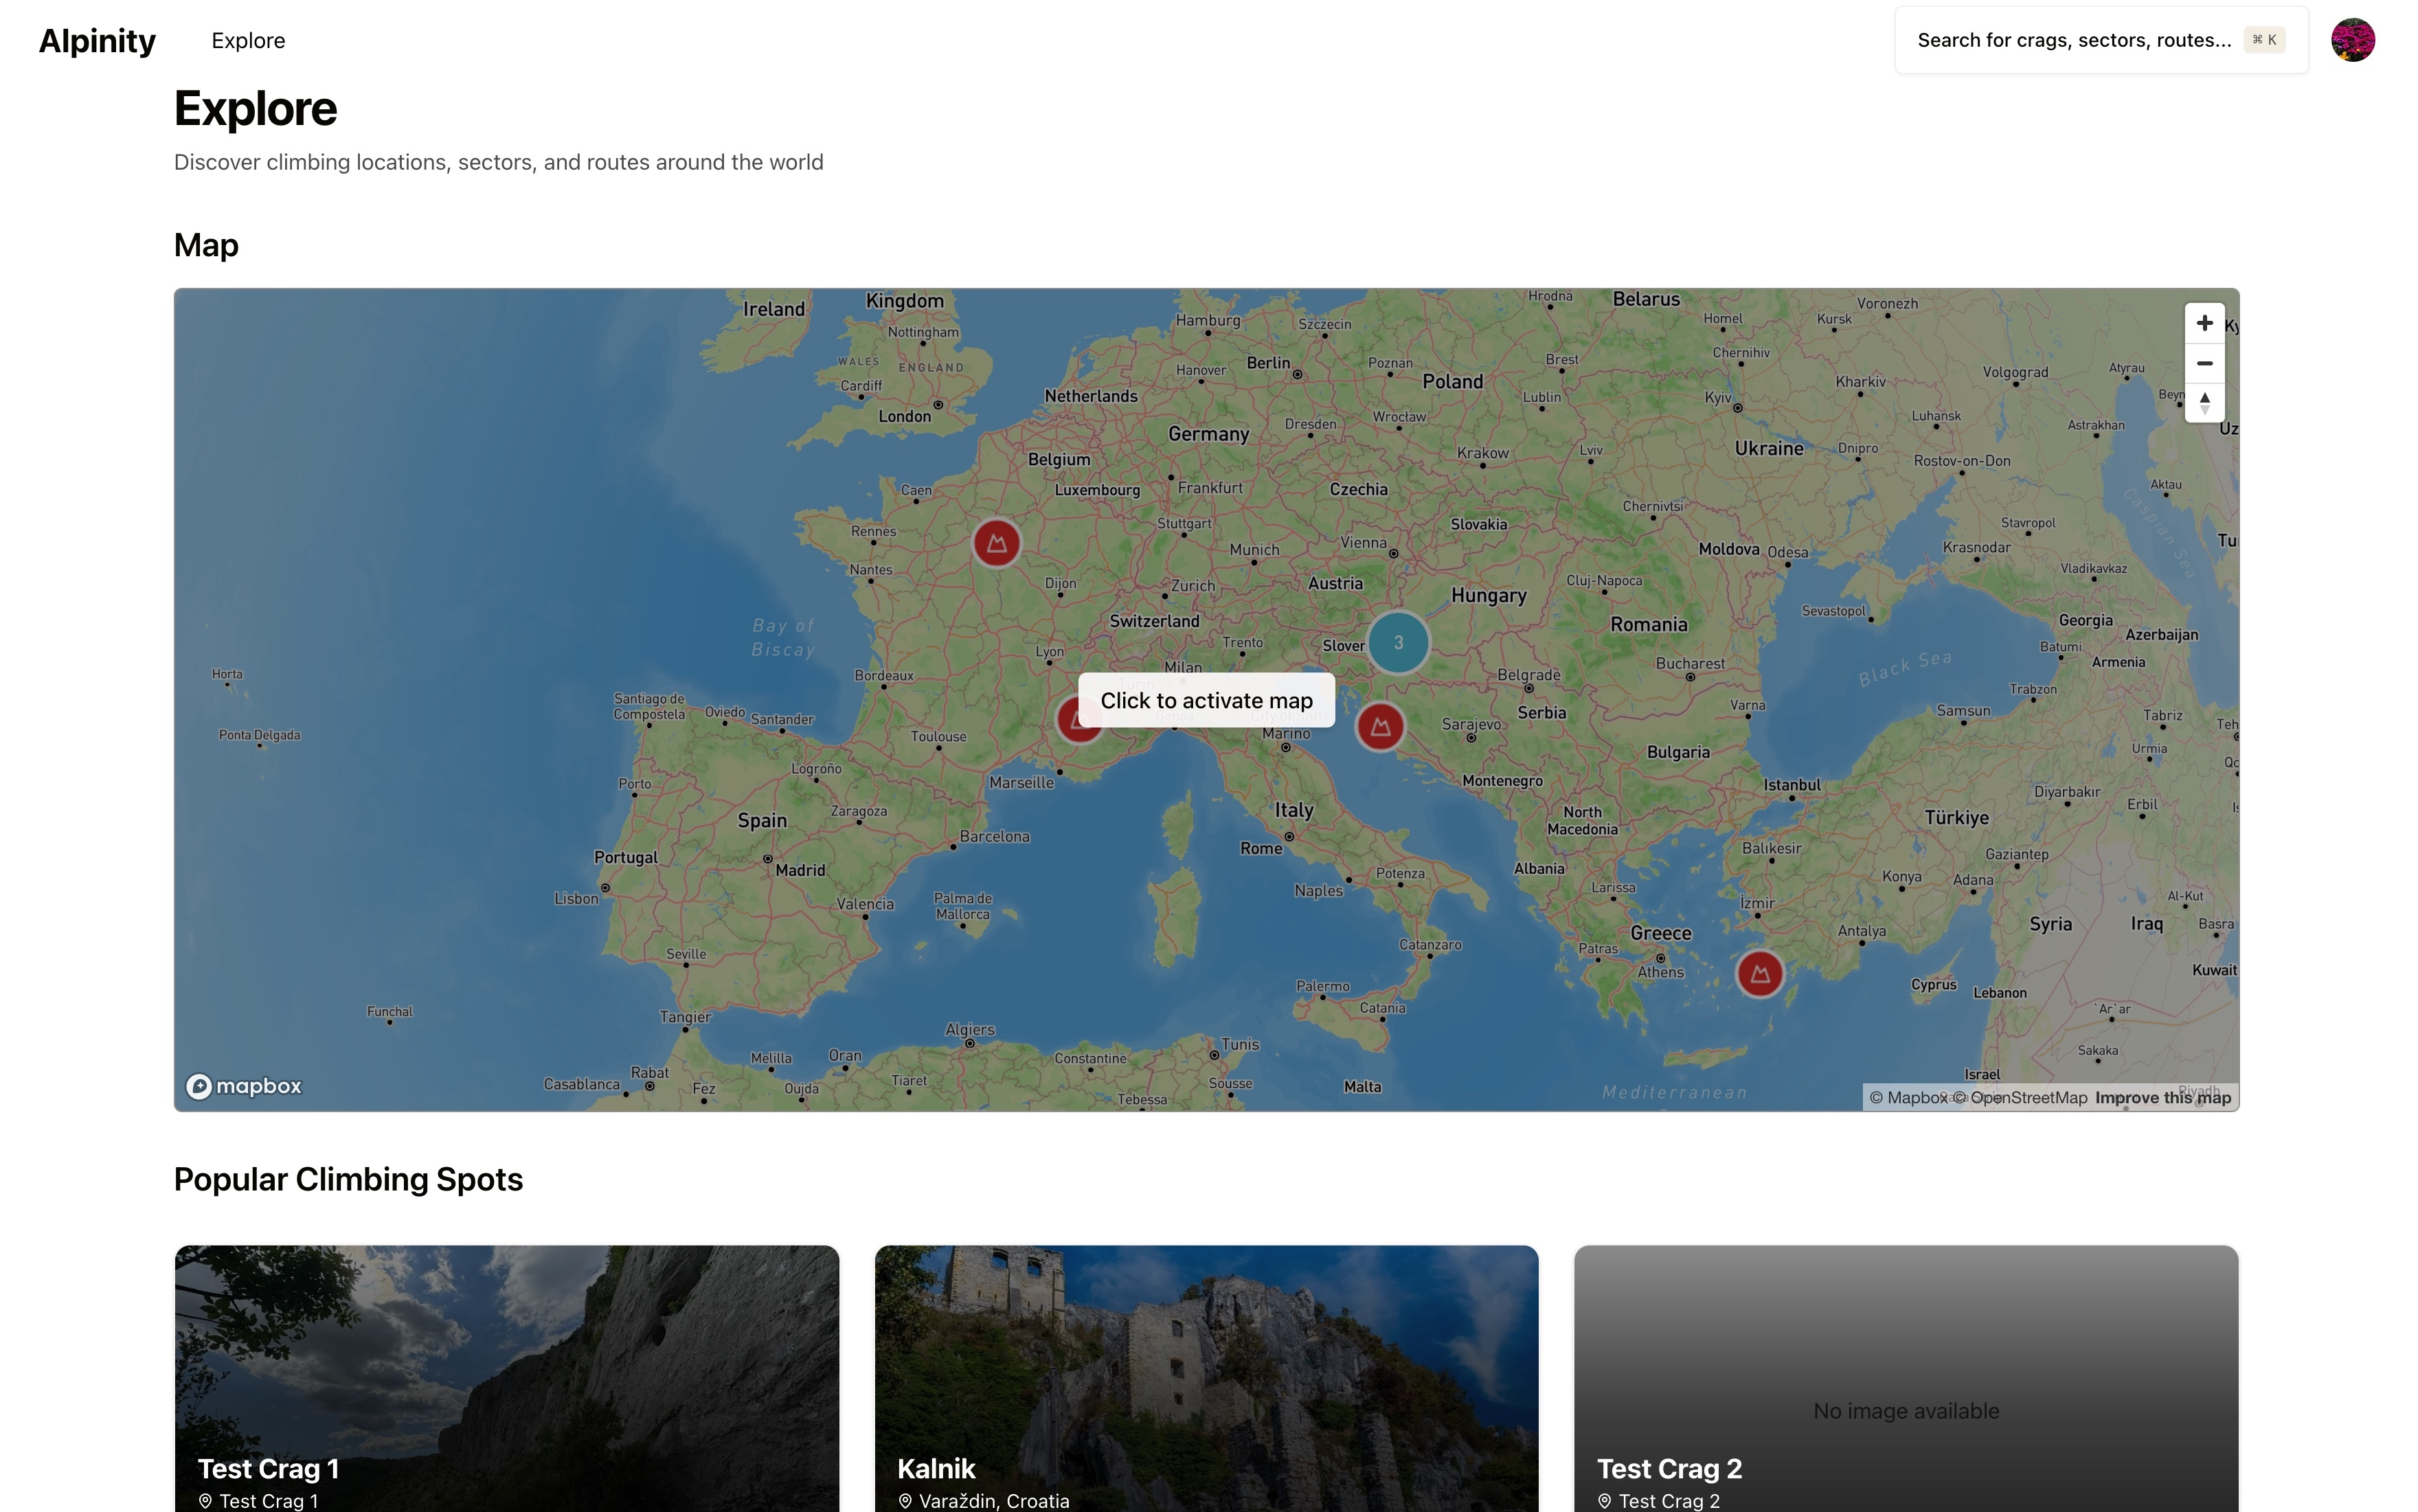
\includegraphics[width=0.9\textwidth]{images/implementacija/web/explore.jpeg}
    \caption{"Istraži" stranica web aplikacije "Alpinity"}
    \label{fig:istrazivanje_web}
\end{figure}